\documentclass[dvipdfmx]{beamer}


%%%%% VIEW %%%%%
\usetheme{Montpellier}
\usecolortheme{crane}
\usefonttheme{professionalfonts} % Math Font
\setbeamertemplate{footline}[frame number] % only frame number in footer
\setbeamertemplate{navigation symbols}{} % remove navigation symbol
\renewcommand{\familydefault}{\sfdefault}% font chenge to Sans-serif in English
\usepackage[deluxe,expert]{otf}
\renewcommand{\kanjifamilydefault}{mg}% font chenge to hiragino in Japanese

\setbeamertemplate{caption}[numbered]
%%%%% Fiture, Table Title Rename %%%%E%
\renewcommand{\figurename}{図}
\renewcommand{\tablename}{表}

\usepackage{bm} % Bold charactor package for math
\usepackage{color}

\usepackage[footnotesize, bf]{caption}
\newcommand{\argmin}{\mathop{\rm arg~min}\limits}

%%%% Definition %%%%%
\usepackage{amsmath,amssymb}
\usepackage{amsthm}
\theoremstyle{definition}

\title{PRML Seminar \#1}
\subtitle{ 1.1-1.6.1 \quad \#PRML学ぼう}
\author{Shunya Ueta}
\institute{Graduate School of SIE, Univ. of Tsukuba \\ Department of Computer Science}
\date{\today} % Print Build time

%%%%% Start Slide part %%%%%

\begin{document}

\begin{frame}
  \titlepage % Generated Title Page by preamble params
\end{frame}

\begin{frame}
  \tableofcontents % Generated tabele of contents by section tag
\end{frame}

\section{Introduction}

\begin{frame}
  \frametitle{自己紹介}
    \begin{itemize}
      \item 名前:上田隼也(@hurutoriya)
      \item 筑波大学大学院1年 Go to Doctor course :)
      \item 情報数理研究室所属
      \item 研究分野 : 画像認識・機械学習
    \end{itemize}
\end{frame}

\subsection{この勉強会について}

\begin{frame}
  \frametitle{この勉強会について}
  \begin{itemize}
    \item パターン認識と機械学習についての輪講です \\
    機械学習とパターン認識の基礎を理解、実用レベルで使いこなす事を目的にセミナーを開催していきます
    \item 2015年を目処に一周予定
    \item 受講者には基礎的な微積分・線形代数・確率統計の知識を前提としています
    \item 資料中のサンプルコードはPythonを採用しています。
    \item 勉強会に関する情報については Hashtag: \textcolor{blue}{\#PRML学ぼう} を使って発信していきます
  \end{itemize}
\end{frame}

\subsection{PRML輪講 \#2 内容}
\begin{frame}
  \frametitle{今回の担当}
  \begin{figure}[htb]
    \centering
    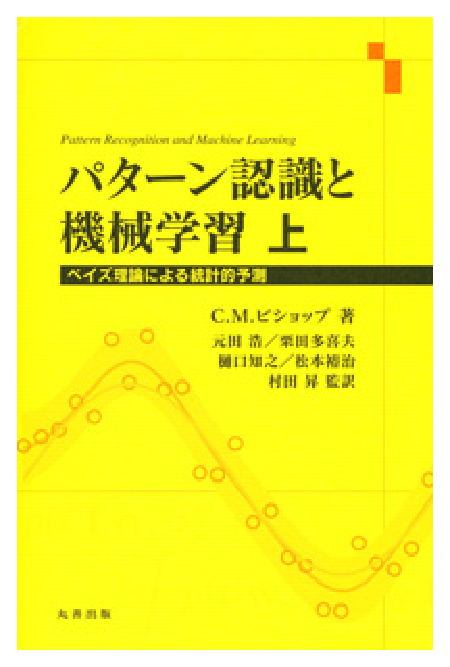
\includegraphics[width=2.5cm,clip]{res/prml.eps}
  \end{figure}
  2$\to$ 2.3.4 
\end{frame}

\section{第$2$章 \enspace 確率分布}
\begin{frame}
  \frametitle{Introduction}
  1章では、確率分布を求める推論が大事だということを証明した。
  
  \textcolor{blue}{密度推定(}density estimation):観測値から確率分布$p(x)$をモデル化
  
  密度推定は基本的に\textcolor{red}{不良設定問題}である。
  
  対象とする観測値$x$において確率分布が$p(x)\neq0$の場合、潜在的に割り当てることができる。
  
  この章では、以下の3つの確率分布を中心に扱っていく。
  \begin{enumerate}
    \item 二項分布
    \item 多項分布
    \item ガウス分布
  \end{enumerate}
\end{frame}

\subsection{2.1 2値変数}
\begin{frame}
  2値確率変数$x={0,1}$を扱う。$x=1$となる確率をパラメータ$\mu$で表す。観測値集合$\bm{D}$の総数は$N$個あり、$x=1$が観測できた回数は$m$回である。
  \begin{gather*}
    p(x=1|\mu) =\mu
  \end{gather*}
  \begin{gather*}
    \rm{Bern}(x|\mu) = \mu^x(1-\mu)^{1-x}
  \end{gather*}
  \begin{gather*}
    \rm{Likelifood} = p(\bm{D}|\mu)= \prod_{n=1}^{N} p(x_n|\mu) = \prod_{n=1}^{N} \mu^{x_n}(1-\mu)^{1-x_n}
  \end{gather*}
  \begin{gather*}
    \mu_{ML} = \frac{m}{N}
  \end{gather*}
\end{frame}

\subsection{2.3 ガウス分布}
\begin{frame}
  \frametitle{Gaussian Distribution}
  変数が一つ, $\mu$は平均,$\sigma^2$は分散を表す。
  \begin{gather*}
     N(x|\mu, \sigma^2) = \frac{1}{\sqrt{2\pi \sigma^2}}\exp\{-\frac{1}{2\sigma^2}(x-\mu)^2 \} 
  \end{gather*}
  変数がD次元ベクトル$\bm{x}$,$\mu$はD次元の平均ベクトル、$\Sigma$は共分散行列を表す。
  \begin{gather*}
     N(x|\mu, \Sigma) = \frac{1}{(2\pi)^{D/2}}\frac{1}{|\Sigma|^{1/2}}\exp\{-\frac{1}{2}(\bm{x}-\mu)^{T} \Sigma^{-1} (\bm{x}-\mu) \} 
  \end{gather*}
\end{frame}

\begin{frame}
  \frametitle{}
\end{frame}

\end{document}
